Una volta concluso lo sviluppo del GRIDS System con Blockchain integrata, è indispensabile valutarne le performance.
Per fare ciò, bisogna selezionare una metrica appropriata...


È stato misurato il tempo che intercorre tra il momento in cui il client effettua la richiesta di data e quello in cui la transazione viene confermata e l'utente può visualizzare i dati.

Una considerazione molto importante da fare è che, nel caso delle transazioni "lente", vi è una sorta di problema di "campionamento": visto che nella Testnet i blocchi vengono estratti ogni circa 20 minuti, il tempo di ritardo varierà in base a quanto tempo prima è stato risolto l'ultimo blocco della blockchain.

Ho provato con 100 transazioni standard e alcune di esse sono state respinte per "error 64: too-long-mempool-chain": non entravano più nel mempool perché ha una misura limitata! Vedere https://www.mycryptopedia.com/mempool-ex plained/ per la spiegazione.

In Bitcoin Core\footnote{https://bitcoin.org/en/bitcoin-core/} il limite di transazioni non confermate che si possono generare di seguito è 25, quindi pazienza. Con bitcoinj non è stato implementato ancora un modo per aggirare questo limite, avrebbe addirittura poco senso, dato che il fatto che i nodi siano in modalità SPV va in antitesi con il fatto di poter generare un numero molto grande di transazioni.

Però in ogni caso la piattaforma ha il meccanismo recharge, quindi il problema non si pone...

Un'altra importante precisazione da fare è che il mempool error si può verificare quando è un singolo wallet a generare troppe transazioni di seguito, non quando sono tanti wallet a generare meno transazioni: ciò significa che la rete SIoT non costituisce \textit{bottleneck}. In condizioni di utilizzo normale da parte di un utente qualsiasi, difficilmente saranno mandate così tante richieste...
%%

Provare con 25 trx "lente"

Poi con 100 trx "veloci" (fatto)

E poi vediamo i tre grafici: ritardo client-side delle trx standard, ritardo totale delle trx standard, ritardo totale delle transazioni veloci.

Sui grafici: 

il client side delay tende ad avere una distribuzione normale (il grafico, infatti, ricorda molto la \textit{normal function}). 

le instant buy presentano ritardi molto contenuti, com'era auspicabile. Da notare il punto con ritardo più alto che corrisponde alla prima richiesta.

l'end-to-end delay, infine, presenta valori temporali molto più ampi, visto che è compreso il tempo della conferma delle transazioni. La discontinuità che si osserva nel grafico è causata dal fatto che una parte delle transazioni sono state incluse in un blocco, mentre un'altra parte è stata confermata nel blocco successivo.

%\begin{figure}[h!t]
%\centerline{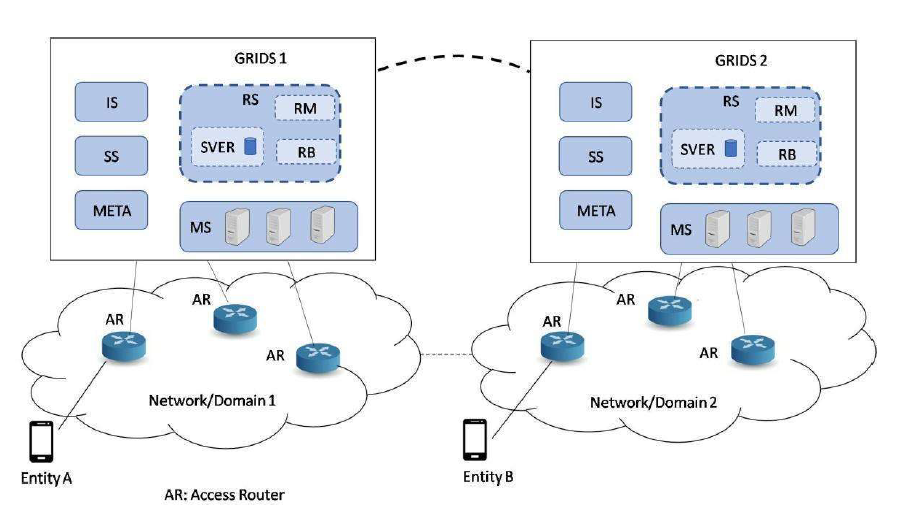
\includegraphics[scale=0.5]{img/GRIDSarch}}
%\caption{Architettura del GRIDS System}
%\label{f:grids:arch}
%\end{figure}